\section{評価}
本章では、提案システムの性能評価について述べる。まず、評価を行う環境について述べる。次に、クラウドゲームサーバ/クライアント間の通信性能の評価について述べる。その後、ゲームプレイ時のフレームレートの評価について述べる。最後に評価についての考察を述べる。

\subsection{評価環境}
既存のクラウドゲーミングシステムはクラウドのデータセンター上でクラウドゲームサーバが動作している。これに対し、提案システムはボランティアが提供する遊休コンピュータ上でクラウドゲームサーバを動作させることで、プレイヤーからデータセンターまでの遅延を削減することを目指した。一般にユーザコンピュータからデータセンターへの遅延は大きくても50ms程度であるが、提案システムでのゲームプレイ中に発生する遅延がこの基準を下回るかどうかを評価する。また、提案システムの通信を実現するために組み込んだトンネリングのオーバヘッドについても評価を行う。

評価を行う環境を図\ref{fig:expenv}のように構築した。ボランティアクラウドゲーミングコントローラは用意せず、クラウドサーバのroma上にはEdgeVPNのリンクを確立するために必要なXMPPサーバのみを用意した。プレイヤーPCの役割を果たすsiciliaではgRPCクライアントとGamingAnywhereクライアントが動作する。また、遊休コンピュータの役割を果たすfirenzeではgRPCサーバ、GamingAnywhereサーバおよびゲームが動作する。siciliaとfirenzeはそれぞれUbuntu20.04で動作するマシンを用い、1Gbpsのリンクを持つネットワークで接続した。このリンクに遅延挿入や帯域制限をかけることで様々なネットワーク環境での評価を実現する。


\begin{figure*}[t]
    \centering
    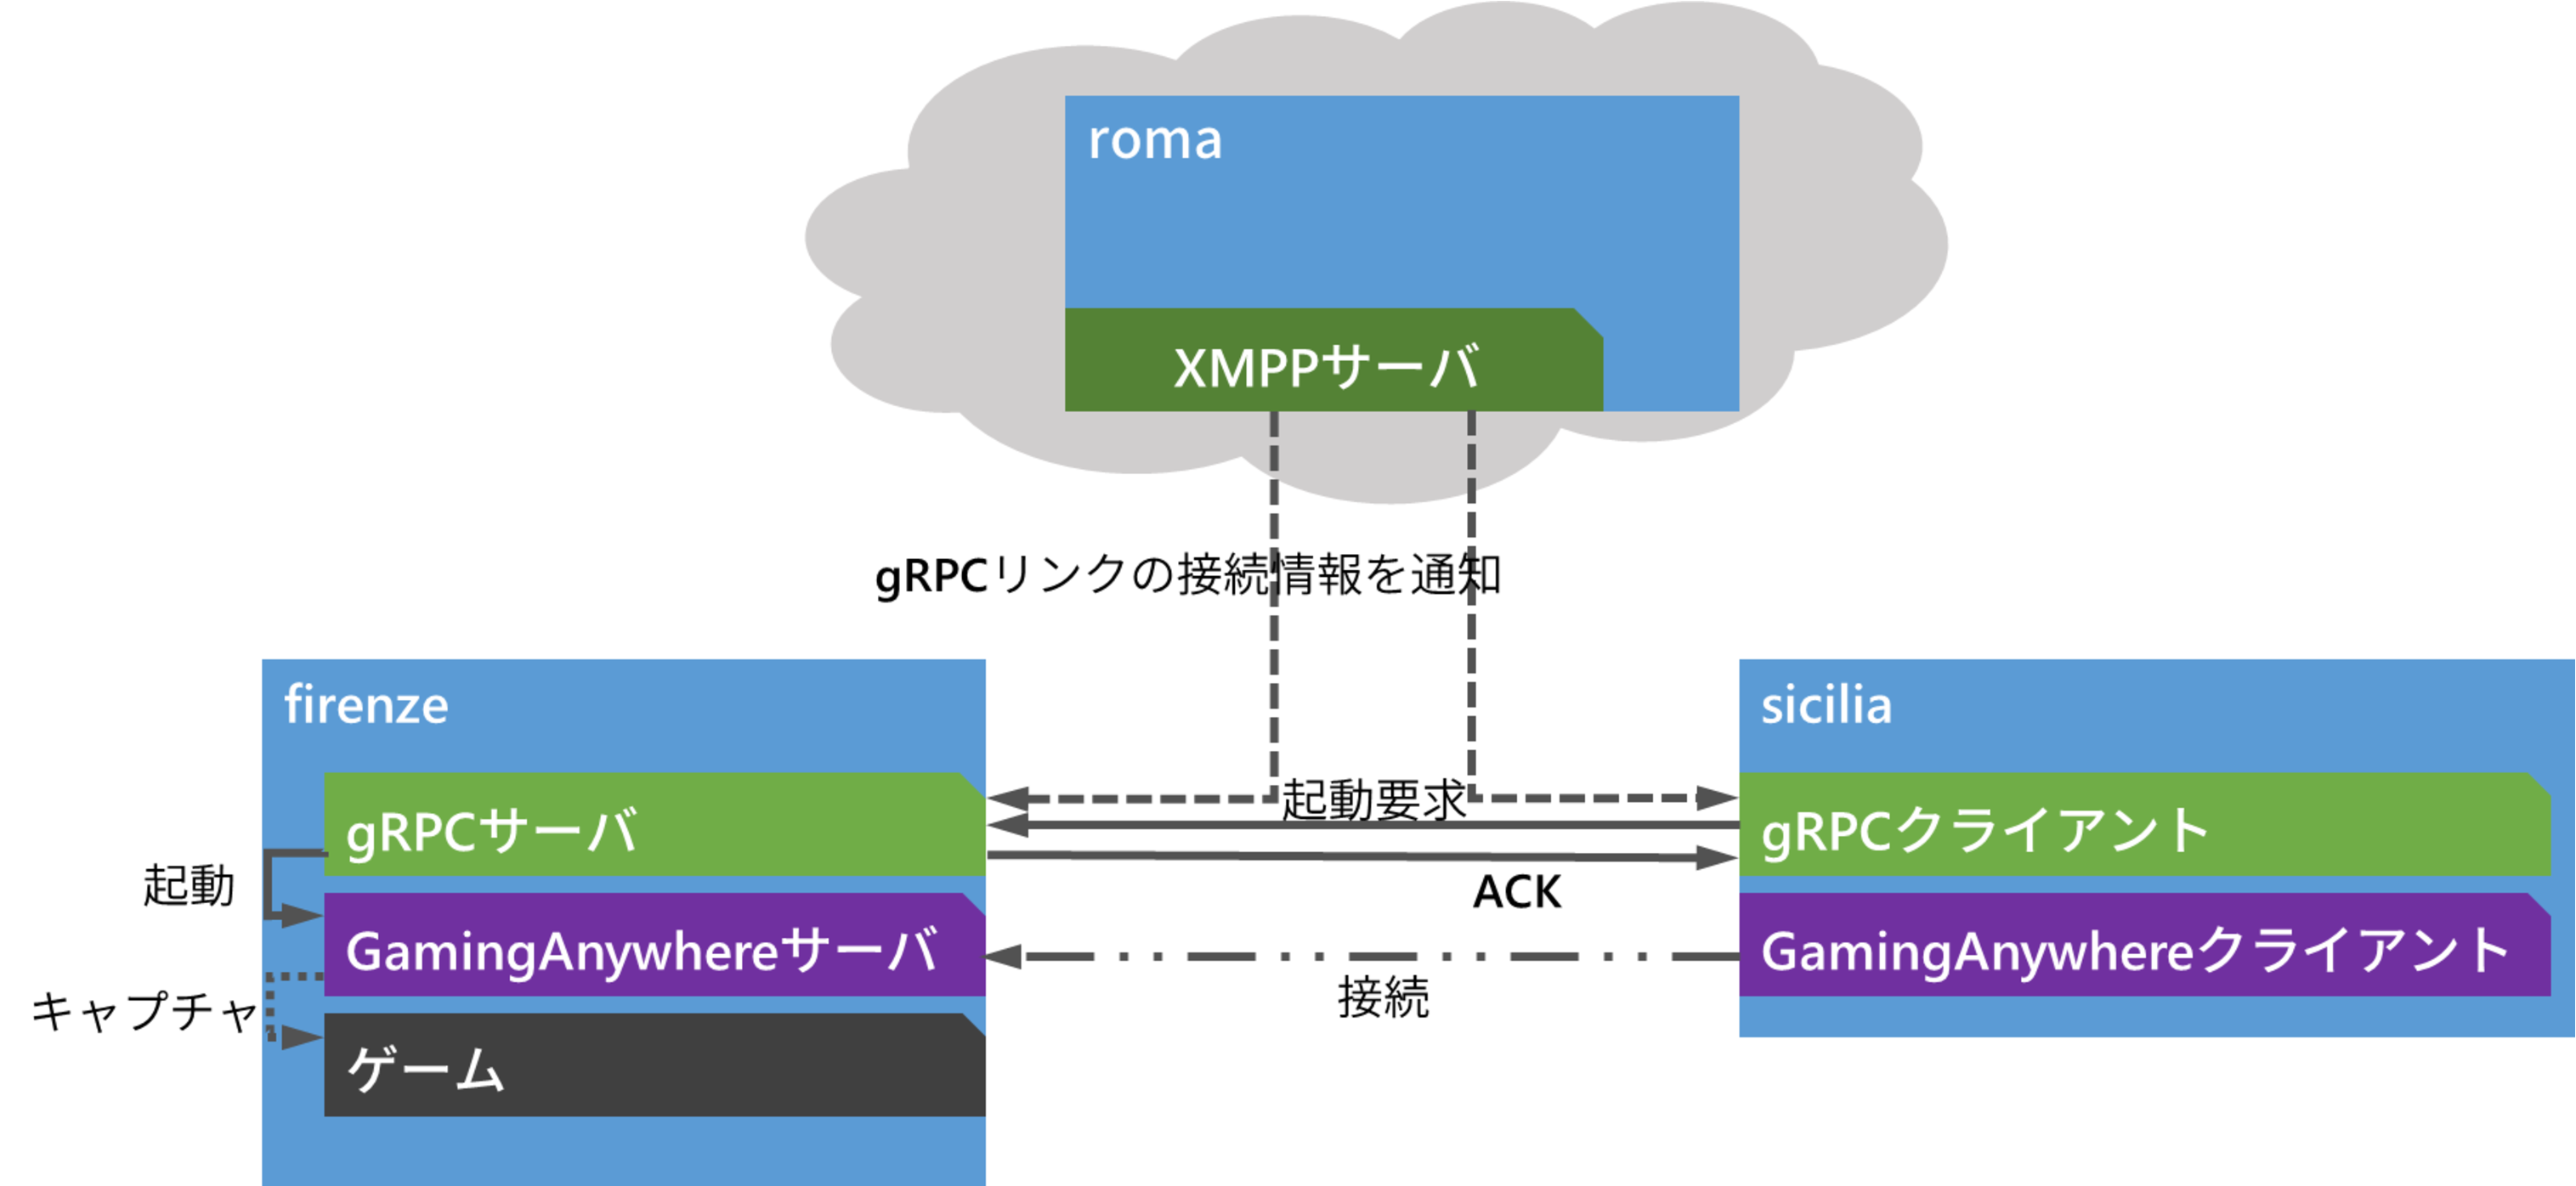
\includegraphics[width=0.8\textwidth,keepaspectratio,clip]{img/experimentalenvironment.eps}
    \caption{評価環境}
    \label{fig:expenv}
\end{figure*}

\subsection{クラウドゲームサーバ/クライアント間の通信性能}

\subsubsection{リンクに対する生の遅延の大小の影響}
tcを使って任意に遅延を挿入し、pingの値で遅延の増え方に影響がないか見る。
遅延が増えたときの遅延の増え方が線形みたいなことを言う。
遅延が増えたときの帯域の減り方の話をする。

\subsubsection{リンクに対する遅延の大小の帯域への影響}
tcを使って任意に遅延を挿入し、iperfで帯域の減り方への影響を見る
遅延が増えたときの帯域の減り方の話をする。

\subsection{ゲームプレイ時のフレームレート}

\subsubsection{ネットワーク帯域の大小の影響}
tcを使って帯域に制限をかけて、実際に複数のゲームをプレイしたときのフレームレートへの影響を見る。
使用したゲームはSteamで公開されているAlbion Online(MMORPG)、Red Eclipse 2(FPS, Action)、Simply Chess(Board Game)

\subsection{考察}
どれぐらい数値が良ければ既存に勝てるのかみたいなこと



\begin{figure*}[t]
    \centering
    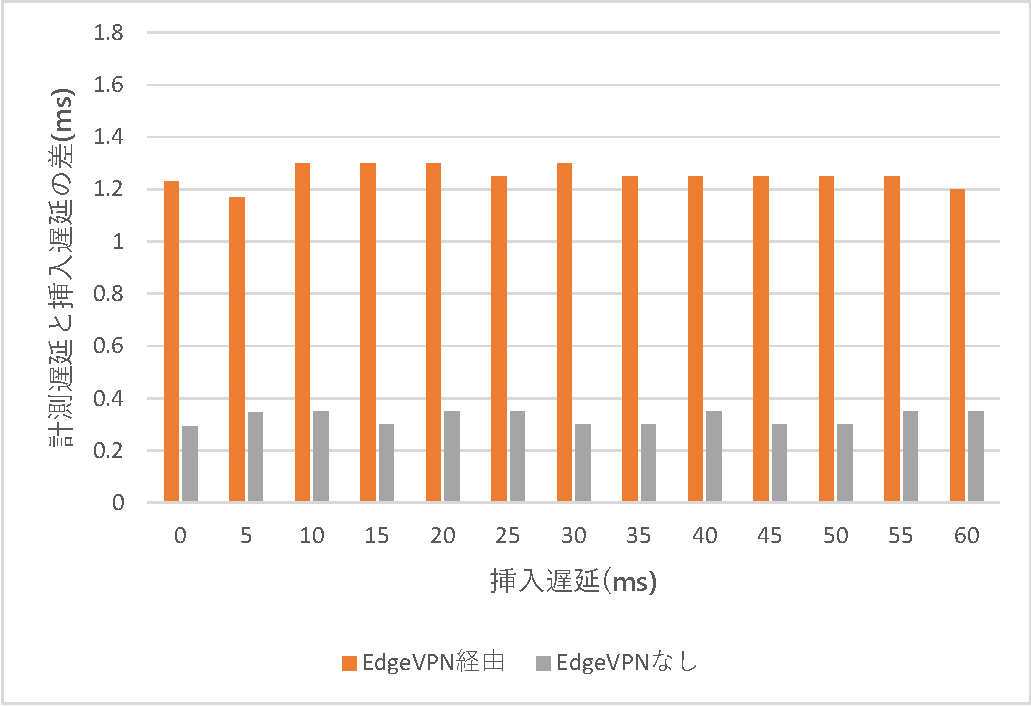
\includegraphics[width=0.8\textwidth,keepaspectratio,clip]{img/graph_ratency.pdf}
    \caption{EdgeVPNリンクに対する遅延挿入の影響}
    \label{fig:ratency}
\end{figure*}

\begin{figure*}[t]
    \centering
    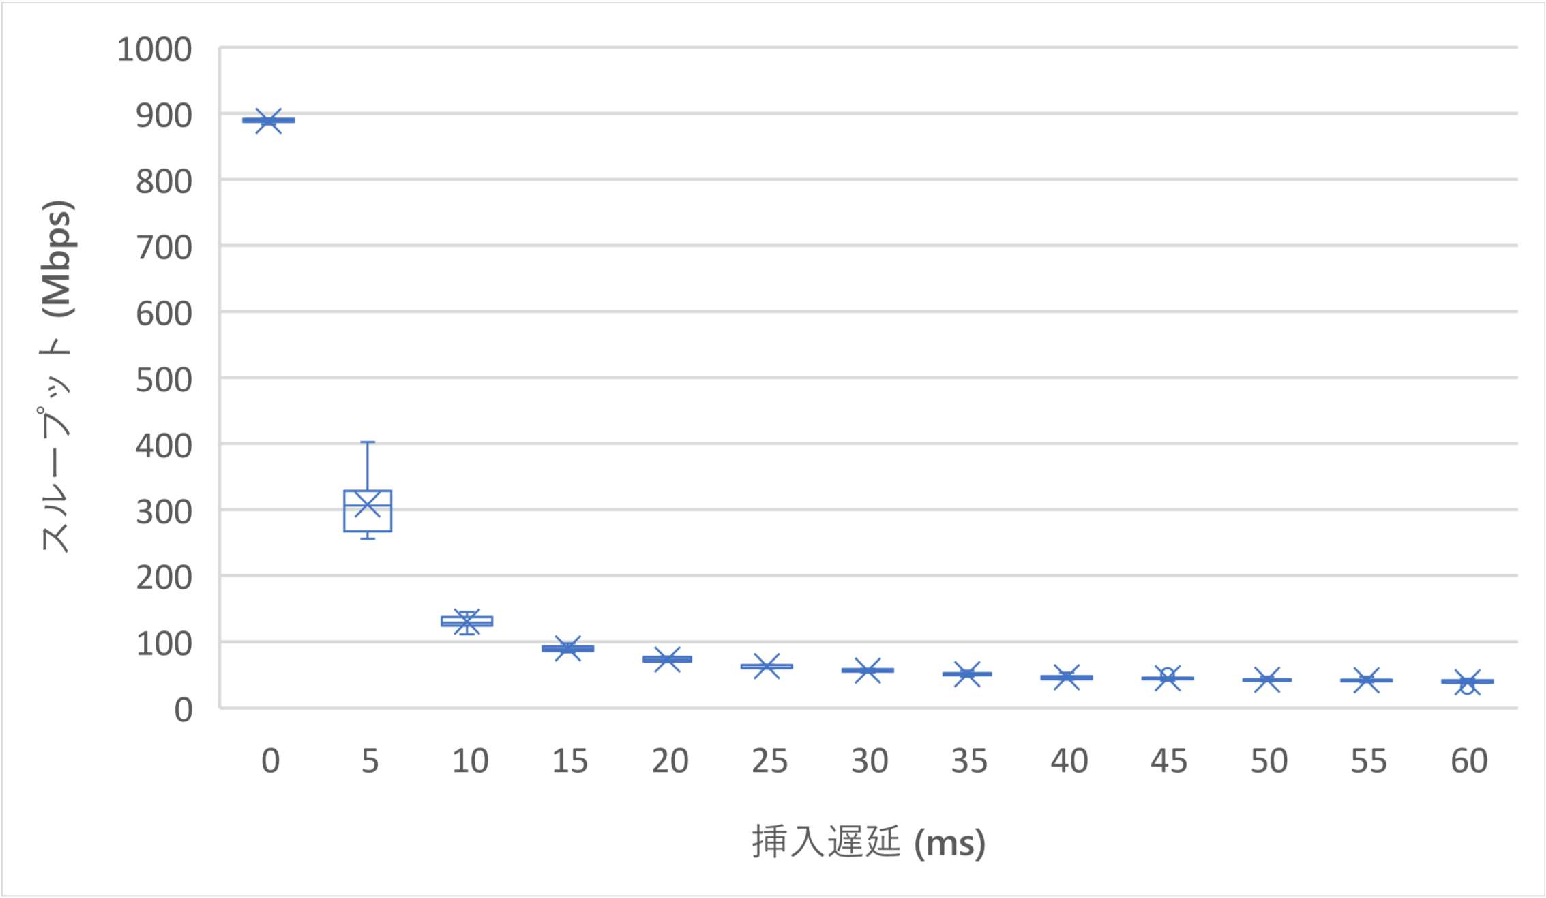
\includegraphics[width=0.8\textwidth,keepaspectratio,clip]{img/bandwidth_withEdgeVPN.pdf}
    \caption{EdgeVPNリンクへの遅延挿入の帯域への影響}
    \label{fig:band_with_edge}
\end{figure*}

\begin{figure*}[t]
    \centering
    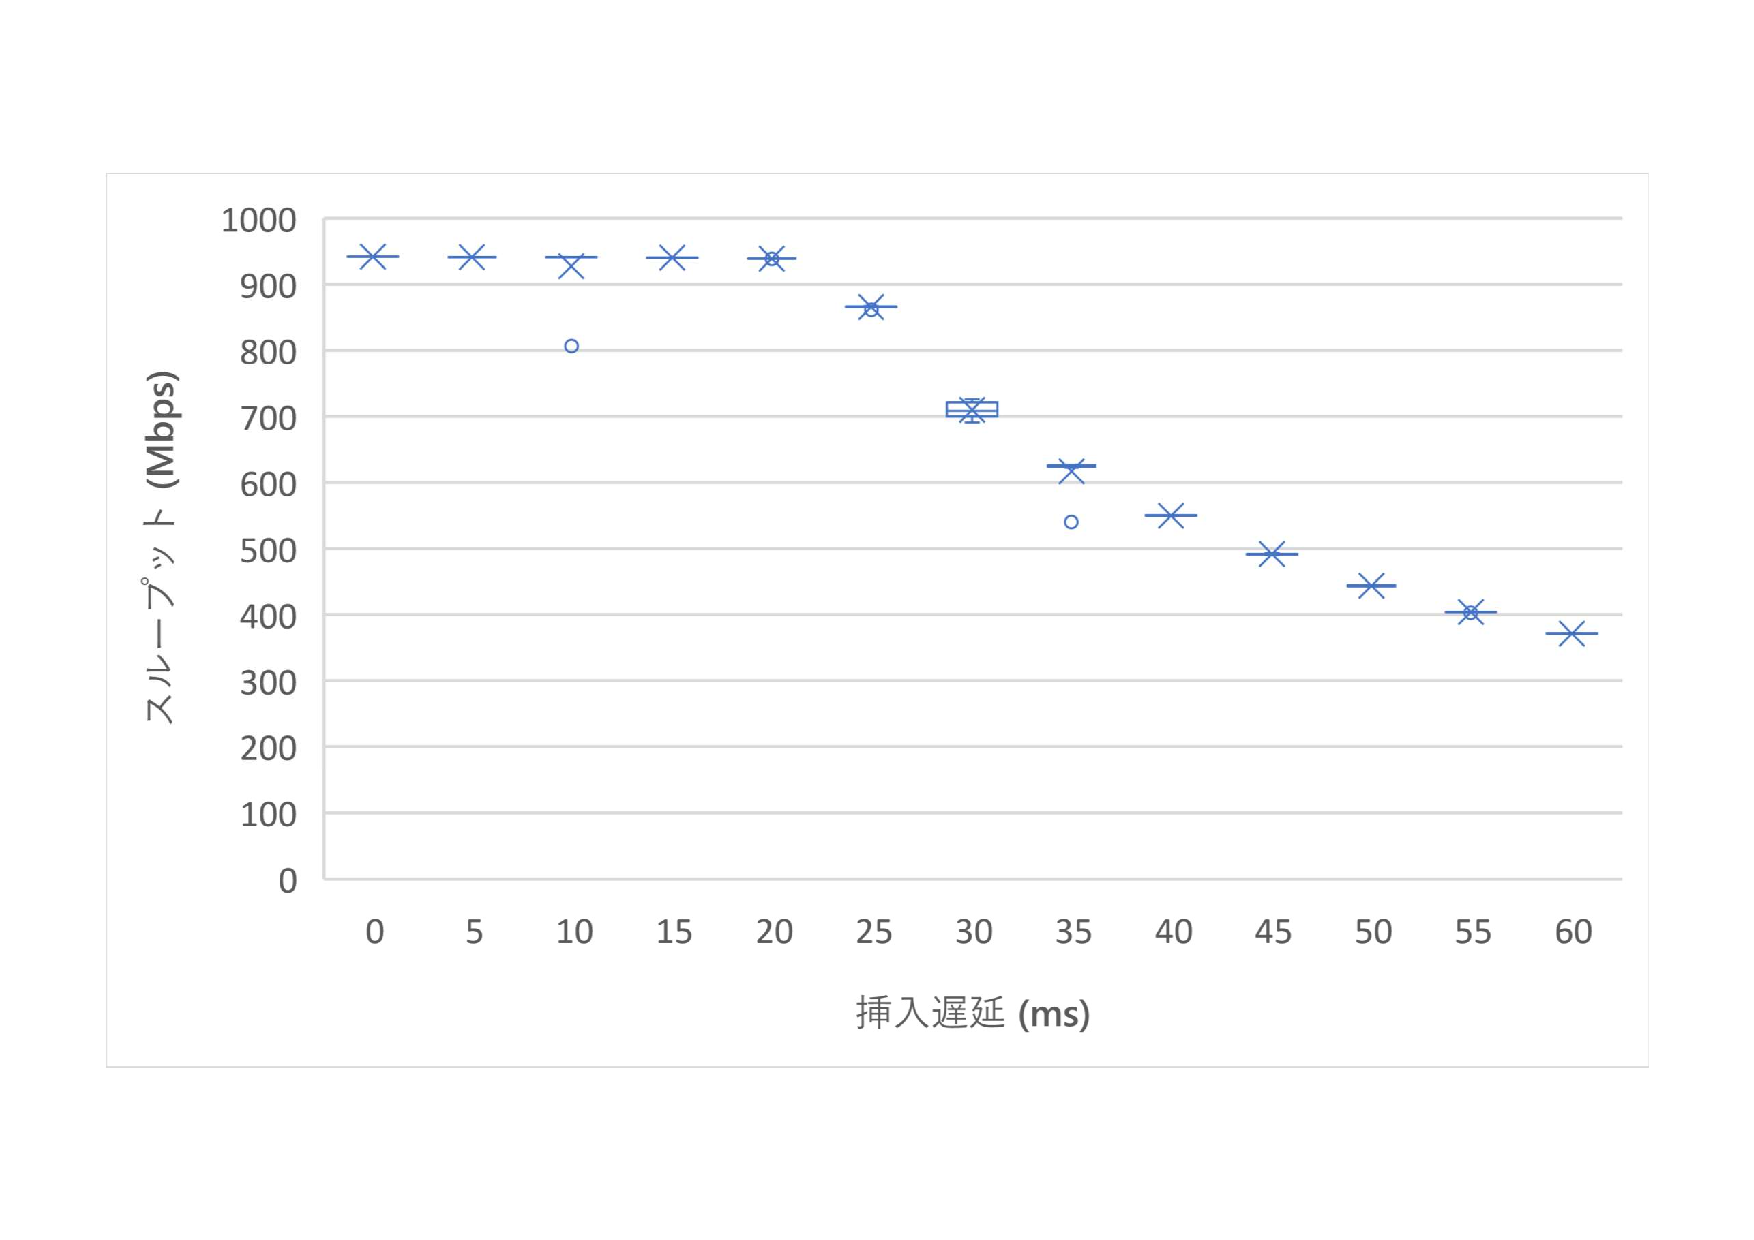
\includegraphics[width=0.8\textwidth,keepaspectratio,clip]{img/bandwidth_withoutEdgeVPN.pdf}
    \caption{EdgeVPNを使用していないリンクへの遅延挿入の帯域への影響}
    \label{fig:band_without_edge}
\end{figure*}

\begin{figure*}[t]
    \centering
    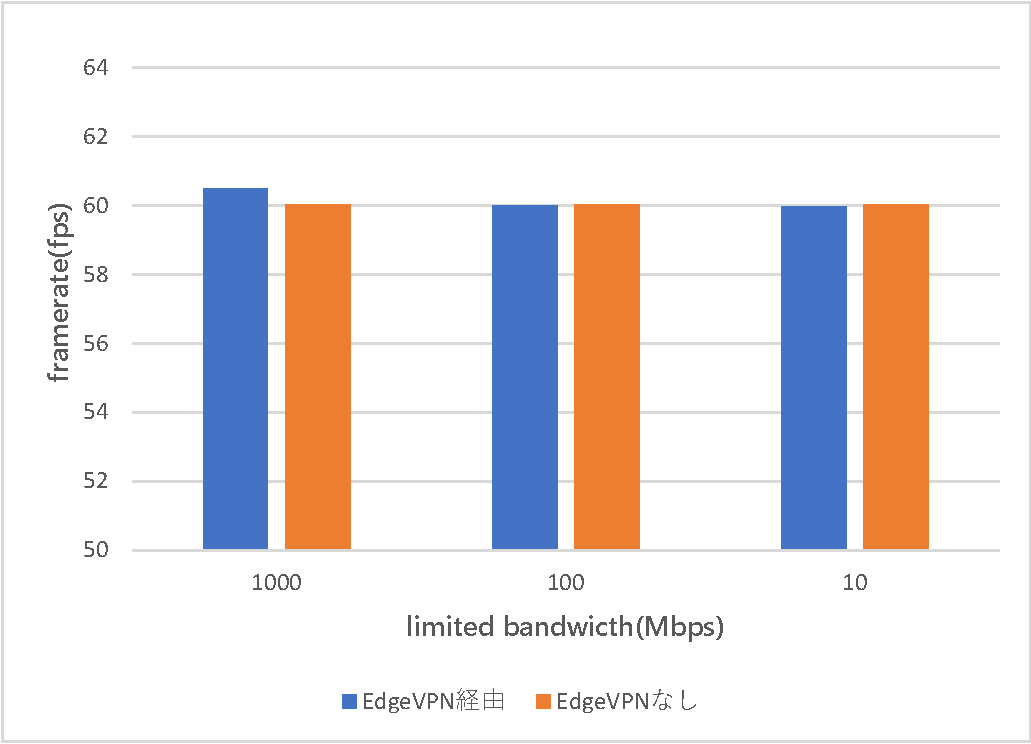
\includegraphics[width=0.8\textwidth,keepaspectratio,clip]{img/framerate_MMO.pdf}
    \caption{帯域制限下でのゲームプレイ時のフレームレートの変化 (Albion Online (MMORPG)プレイ時)}
    \label{fig:fps_mmo}
\end{figure*}

\begin{figure*}[t]
    \centering
    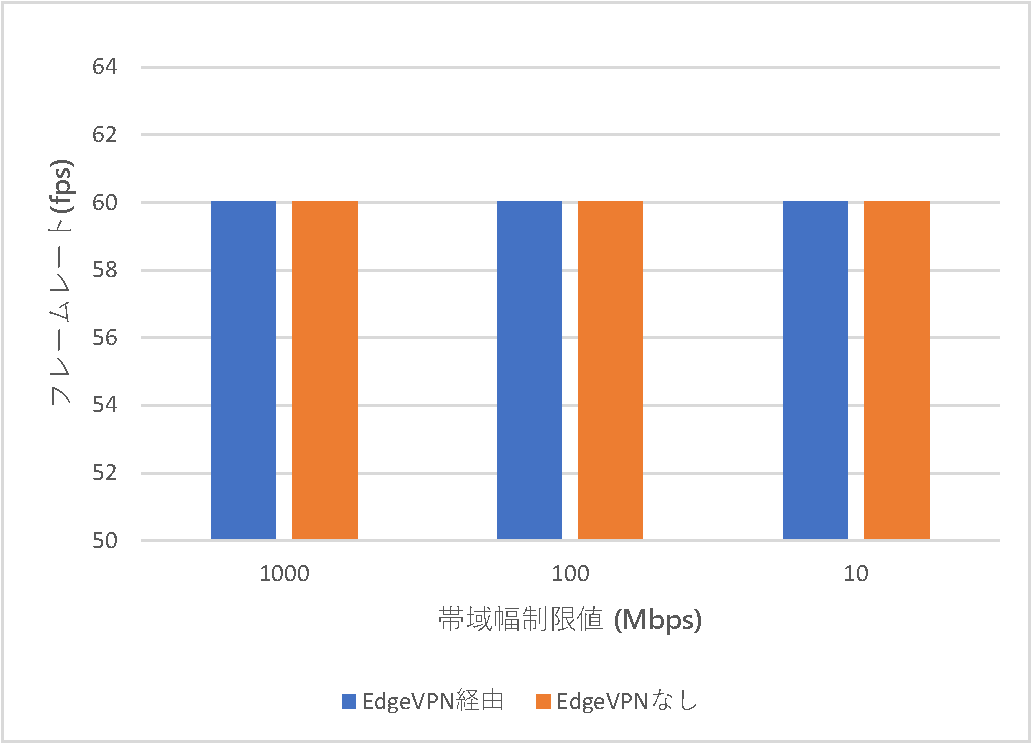
\includegraphics[width=0.8\textwidth,keepaspectratio,clip]{img/framerate_FPS.pdf}
    \caption{帯域制限下でのゲームプレイ時のフレームレートの変化 (Red Ecliplse 2 (FPS, Action)プレイ時)}
    \label{fig:fps_fps}
\end{figure*}

\begin{figure*}[t]
    \centering
    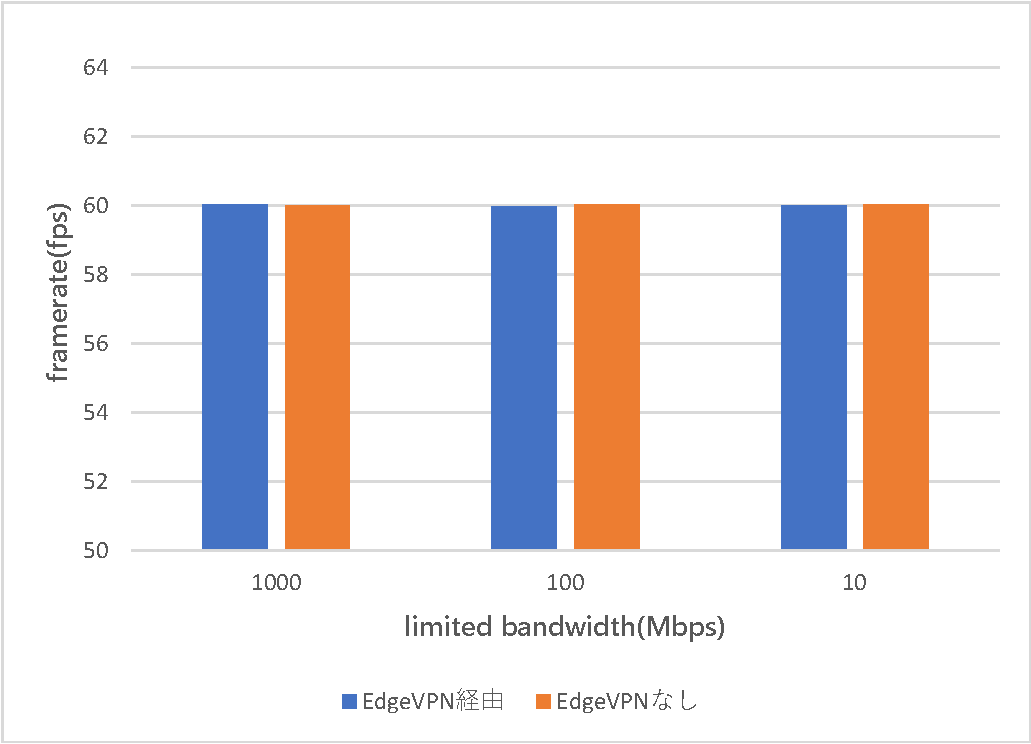
\includegraphics[width=0.8\textwidth,keepaspectratio,clip]{img/framerate_Board.pdf}
    \caption{帯域制限下でのゲームプレイ時のフレームレートの変化 (Simply Chess (ボードゲーム)プレイ時)}
    \label{fig:fps_board}
\end{figure*}